\section{Protocol and Local-Observation Model}
\label{sec:model}

\subsection{DB-LBT Insertion Point}

Let $\mathcal K=\mathcal K_{\rm W}\cup\mathcal K_{\rm N}$ contain the Wi-Fi
APs and NR-U gNBs sharing one channel. For local countdown slot $\ell$, node
$k$ updates
\begin{equation}
c_k(\ell+1)=
\begin{cases}
c_k(\ell)-1, & C_k(\ell)=0,\\
c_k(\ell), & C_k(\ell)=1,
\end{cases}
\label{eq:countdown}
\end{equation}
where $C_k=1$ is a busy CCA sample. A maximal busy episode freezes the
counter and increments interruption count $i_k$. In a mutually detectable
collision domain, successful peer transmissions create distinct busy episodes,
which motivates the DB-LBT estimate $\hat n_k\approx 1+i_k$.

\begin{figure}[!t]
  \centering
  \subfloat[Local observation and action boundary.]{%
    \resizebox{\columnwidth}{!}{\begin{tikzpicture}[
  font=\footnotesize,
  node distance=4mm,
  block/.style={draw,rounded corners=1.5pt,align=center,minimum height=8mm,inner sep=2.5pt,text width=48mm},
  env/.style={block,fill=gray!10},
  obs/.style={block,fill=cyan!9},
  learn/.style={block,fill=orange!12},
  protocol/.style={block,fill=green!10},
  arrow/.style={-{Latex[length=2mm]},thick}
]
\node[env] (env) {Radio environment\\$G_{jk}(t)$, traffic, other transmitters};
\node[obs,below=of env] (cca) {Native sensing and decoding\\$C_k(t)$, ACK/HARQ $Y_k(t)$};
\node[obs,below=of cca] (ctx) {Local history\\busy, interruptions, delay, queue, retries};
\node[learn,below=of ctx] (agent) {Independent LinUCB\\select $(\kappa,\beta,m,b_{\rm init})$};
\node[protocol,below=6mm of agent] (mac) {Unchanged access protocol\\Wi-Fi EDCA or NR-U Cat-4 LBT};

\draw[arrow] (env) -- (cca);
\draw[arrow] (cca) -- (ctx);
\draw[arrow] (ctx) -- (agent);
\draw[arrow] (agent) -- node[midway,right=1mm,align=left,font=\tiny,
  fill=white,inner sep=0.5pt]{next recovery\\profile only} (mac);
\draw[arrow] (mac.east) -- ++(8mm,0) |- node[pos=.25,right]{future attempts} (env.east);

\node[draw,dashed,rounded corners=1.5pt,fit=(cca)(ctx)(agent)(mac),inner sep=2.5mm,
  label={[align=center,font=\scriptsize]below:{Fixed outside learning: ED threshold, AIFS/defer, slot duration,\\MCOT, synchronization, MCS, and HARQ}}] {};
\end{tikzpicture}
}}\\[-1mm]
  \subfloat[Insertion point in Wi-Fi and NR-U access.]{%
    \resizebox{\columnwidth}{!}{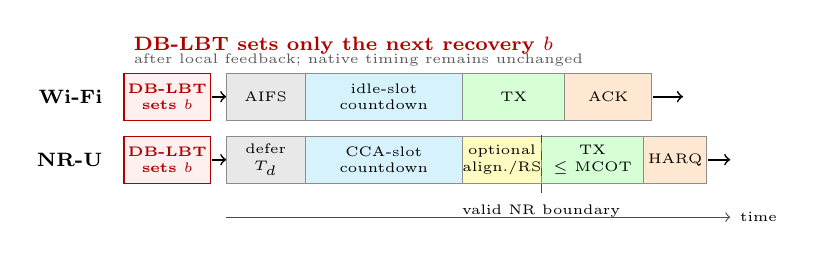
\begin{tikzpicture}[font=\scriptsize,x=1mm,y=1mm]
\tikzset{
  phase/.style={draw=black!45,minimum height=6mm,inner sep=0pt,
    align=center,text=black,font=\tiny},
  learned/.style={phase,draw=red!70!black,fill=red!6,
    text=red!70!black,font=\tiny\bfseries},
  native/.style={phase,fill=gray!18},
  countdown/.style={phase,fill=cyan!16},
  transmit/.style={phase,fill=green!16},
  feedback/.style={phase,fill=orange!18},
  alignment/.style={phase,fill=yellow!24}
}

\node[anchor=west,text=red!70!black,font=\scriptsize\bfseries]
  at (10,18.5) {DB-LBT sets only the next recovery $b$};
\node[anchor=west,text=black!65,font=\tiny]
  at (10,16.7) {after local feedback; native timing remains unchanged};

\node[anchor=east,font=\scriptsize\bfseries] at (8.5,12) {Wi-Fi};
\node[learned,minimum width=11mm] at (15.5,12) {DB-LBT\\sets $b$};
\draw[->,semithick] (21.2,12) -- (23,12);
\node[native,minimum width=10mm] at (28,12) {AIFS};
\node[countdown,minimum width=20mm] at (43,12) {idle-slot\\countdown};
\node[transmit,minimum width=13mm] at (59.5,12) {TX};
\node[feedback,minimum width=11mm] at (71.5,12) {ACK};
\draw[->,semithick] (77.2,12) -- (81,12);

\node[anchor=east,font=\scriptsize\bfseries] at (8.5,4) {NR-U};
\node[learned,minimum width=11mm] at (15.5,4) {DB-LBT\\sets $b$};
\draw[->,semithick] (21.2,4) -- (23,4);
\node[native,minimum width=10mm] at (28,4) {defer\\$T_d$};
\node[countdown,minimum width=20mm] at (43,4) {CCA-slot\\countdown};
\node[alignment,minimum width=10mm] at (58,4) {optional\\align./RS};
\node[transmit,minimum width=13mm] at (69.5,4) {TX\\$\leq$ MCOT};
\node[feedback,minimum width=8mm] at (80,4) {HARQ};
\draw[->,semithick] (84.2,4) -- (87,4);

\draw[dashed,black!70] (63,-0.2) -- (63,7.2);
\node[anchor=north,align=center,text=black,font=\tiny] at (63,-0.5)
  {valid NR boundary};
\draw[->,black!70] (23,-3.3) -- (87,-3.3)
  node[anchor=west,text=black,font=\tiny] {time};
\end{tikzpicture}
}}
  \caption{Each transmitter selects only its next DB-LBT recovery profile.
  Native CCA, countdown, synchronization, MCOT, and ACK/HARQ behavior remain
  outside the learner.}
  \label{fig:protocol}
\end{figure}

Figure~\ref{fig:protocol} locates the control boundary. DB-LBT supplies the
next recovery counter after an ACK/HARQ outcome. Wi-Fi still applies its
inter-frame deferral and EDCA rules; NR-U still applies its priority class,
maximum channel occupancy, and transmission-boundary alignment
\cite{kosek2021downlink,3gpp37213}.

\subsection{What Local History Can Represent}

Propagation gain $G_{jk}(t)$ includes path loss, shadowing, and small-scale
fading. CCA and reception compress that nonlinear channel into protocol
outcomes:
\begin{align}
C_k(t)&=\mathbb 1\!\left\{N_k+\sum_{j\ne k}a_j(t)P_jG_{jk}(t)
\geq\Gamma_k\right\},
\label{eq:cca}\\
\Pr\{Y_k=1\mid\gamma_k,u_k\}
&=1-\mathrm{PER}_{\tau_k}(\gamma_k,u_k).
\label{eq:success}
\end{align}
A failed packet can thus result from simultaneous access, fading, hidden
interference, or decoding. The learner never treats one failure as a collision
measurement.

Three conditions connect these outcomes to the event-level contention model:
(A1) every co-channel transmission exceeds every contender's CCA threshold;
(A2) isolated reception succeeds with high probability; and (A3) simultaneous
transmissions have no capture. Then
\begin{equation}
\begin{aligned}
C_k(\ell)&=\mathbb 1\!\left\{\sum_{j\ne k}a_j(\ell)>0\right\},\\
Y_k(\ell)&=1\iff\sum_j a_j(\ell)=1.
\end{aligned}
\label{eq:reduction}
\end{equation}
Busy episodes now carry contention information: one zero counter succeeds and
multiple zeros collide. Equation~\eqref{eq:reduction} is an abstraction for
the event experiment, not a claim that a fading PHY is linear.

The controller aggregates 11 measurements already available at an AP or gNB:
success and failure ratios, CCA busy fraction, countdown interruptions, delay
EWMA and P95, queue occupancy, arrivals, retransmissions, effective-data
occupancy, and $\hat n_k=\operatorname{clip}(1+\bar i_k,1,32)$. CCA and
interruptions indicate occupancy; queue and delay reveal demand; ACK/HARQ and
retransmissions describe service after access. Periodic occupancy or a changed
active set need not be explicitly labeled if it leaves a distinct local trace.

\begin{table}[!t]
\caption{Local Features and Their Protocol Origin}
\label{tab:context}
\centering
\scriptsize
\begin{tabularx}{\columnwidth}{@{}p{19mm}p{24mm}Y@{}}
\toprule
Feature group & Local source & Action-relevant cue \\
\midrule
Busy fraction, interruptions & CCA and countdown freezes & Active peers or persistent occupancy \\
Success, failure, retries & ACK/HARQ and retry state & Service after attempted access \\
Queue, arrivals, delay & Local traffic and MAC queue & Activation and congestion \\
Effective-data occupancy, busy share & Successful channel use & Schedule efficiency and local share \\
\bottomrule
\end{tabularx}
\end{table}

Let $z$ denote a MAC occupancy regime, $q^\star(z)$ its best allowed profile,
and $\bar x_k(z)$ node $k$'s mean context. Action-relevant local separability
requires
\begin{equation}
q^\star(z)\ne q^\star(z')\Longrightarrow
\|\bar x_k(z)-\bar x_k(z')\|_2\geq\delta_x>0.
\label{eq:identifiability}
\end{equation}
The corresponding timescales are
\begin{equation}
T_{\rm phy}\ll T_{\rm ctx}\lesssim T_{\rm adapt}
\ll T_{\rm dwell}<T_{\rm hor}.
\label{eq:timescale}
\end{equation}
Fast radio and arrival randomness can then average into history before a phase
changes, while at least one change occurs within the operating horizon.
Equations~\eqref{eq:identifiability}--\eqref{eq:timescale} define the difficult
but testable setting in which local adaptation is useful.
